% Chapter X

\chapter{Extracting biological signal from contact maps} % Chapter title

\label{ch:02-01} % For referencing the chapter elsewhere, use \autoref{ch:name} 

%----------------------------------------------------------------------------------------

Most genomics methods generate a large amount of data. The information contained in these data is not always readily accessible, and in addition most of it is often not directly relevant for the problem at hand. One of the main challenges emanating from genomics data is therefore process the data to extract meaningful information, and then distill this information and extract only the relevant signal.

In the case of Hi-C and other related derivative genomics techniques, the resulting signal is a collection of contacts recorded between pairs of genomic segments. These contacts reflect the average genome structure from a population of cells. However, in addition to reflecting the average of a population of cells, the data themselves are subject to various biases intrinsic to their generation.

The specific contacts revealing spatial features and changes of interest are therefore sometimes hard to detect and, importantly, to quantify and validate statistically. They can be faint, reflecting events that occur only in a fraction of the cells in the population, or masked by experimental noise. This is especially true regarding data generated from species that are not heavily investigated and for which optimization of the protocols was not performed. The quality of the data has indeed strongly improved over the last 10 years, allowing to reduce bin sizes from 1 Mb for a human contact map in 2009 \cite{lieberman-aidenComprehensiveMappingLongRange2009}, to 1 kb in more recent papers. In yeast, bacteria, or Archaea, several years passed before protocols reaching a decent resolution (e.g. \textasciitilde 20 kb bin) were developed. Only recently contact maps of bacteria reached bin sizes of 1 kb \cite{cockramGenerationGenelevelResolution2021}. Detecting and quantifying the changes in these contact maps of variable quality therefore requires a set of bias correction and signal detection methods which are still under continuous development, drawing from innovation in computer science and algorithmic fields.

In this section we review the recent methodological developments that allow to correct the Hi-C signal and present new methods to extract, quantify and assess the relevance of biological features from these datasets. These developments proved necessary to tackle the questions raised in the following chapters.


\section{Streamlined and reproducible Hi-C processing}
\label{sec:02-01:streamlined-processing}
% Existing methods: painful to install, non tested (risky), non reproducible
% hicstuff, hicreppy

Pre-processing of Hi-C data, which consists in converting \acrfull{NGS} reads into chromosomal contact matrices involves several steps that will impact the resulting signal. The sequencing reads themselves can be the result from religation of two distinct loci (Fig. \ref{fig:02-01:chimeric}). These chimeric reads cannot be aligned reliably with generic methods and need to be cut for proper alignment \cite{lajoieHitchhikerGuideHiC2015}. Chimeric reads become more problematic when increasing the read size relative to restriction fragment length.

\begin{figure}[htb]
    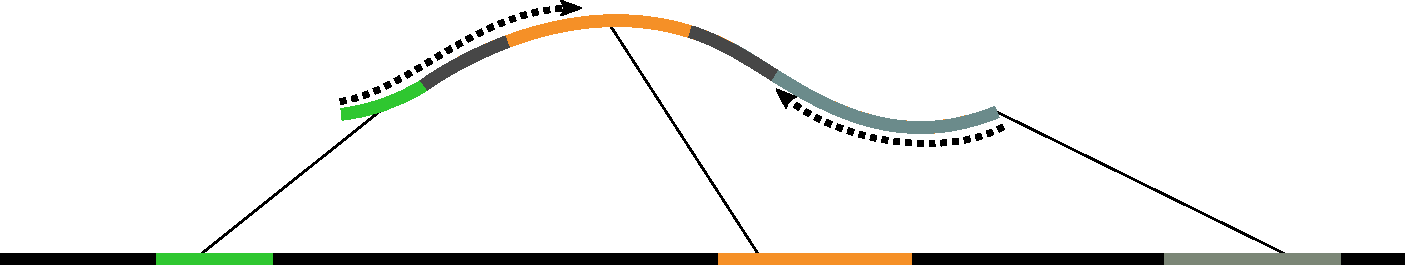
\includegraphics[width=0.8\textwidth]{Parts/Part02/gfx/hicstuff/chimeric.pdf}
    \caption[Chimeric reads in Hi-C.]{Chimeric reads in Hi-C: Example of a Hi-C fragment resulting in a chimeric read. The Hi-C fragment contains 3 different regions (green, orange and grey) which have been religated together. The paired-end sequencing reads are shown as dotted line. The sequencing read spanning the green and orange region will be chimeric and not map to a unique region.}
    \label{fig:02-01:chimeric}
\end{figure}

Not all read pairs generated by Hi-C experiments represent valid spatial interactions. Some restriction fragments are sequenced without religation and other fragments religate on themselves (Fig. \ref{fig:02-01:filters}) \cite{cournacNormalizationChromosomalContact2012}. The various interaction types can be separated based on the strand of origin of their individual reads. In theory, and in practice at long ranges, one would expect religations to be strand agnostic and to have an equal abundance of all four possible combinations ($++$, $--$, $+-$, $-+$). In reality, this is never the case at short range contacts, due to the enrichment of dangling ends (or uncut fragments, $+-$) and self-circles (or loops, $-+$) (Fig. \ref{fig:02-01:filters}b, c) \cite{cournacNormalizationChromosomalContact2012}.

\begin{figure}[htb]
    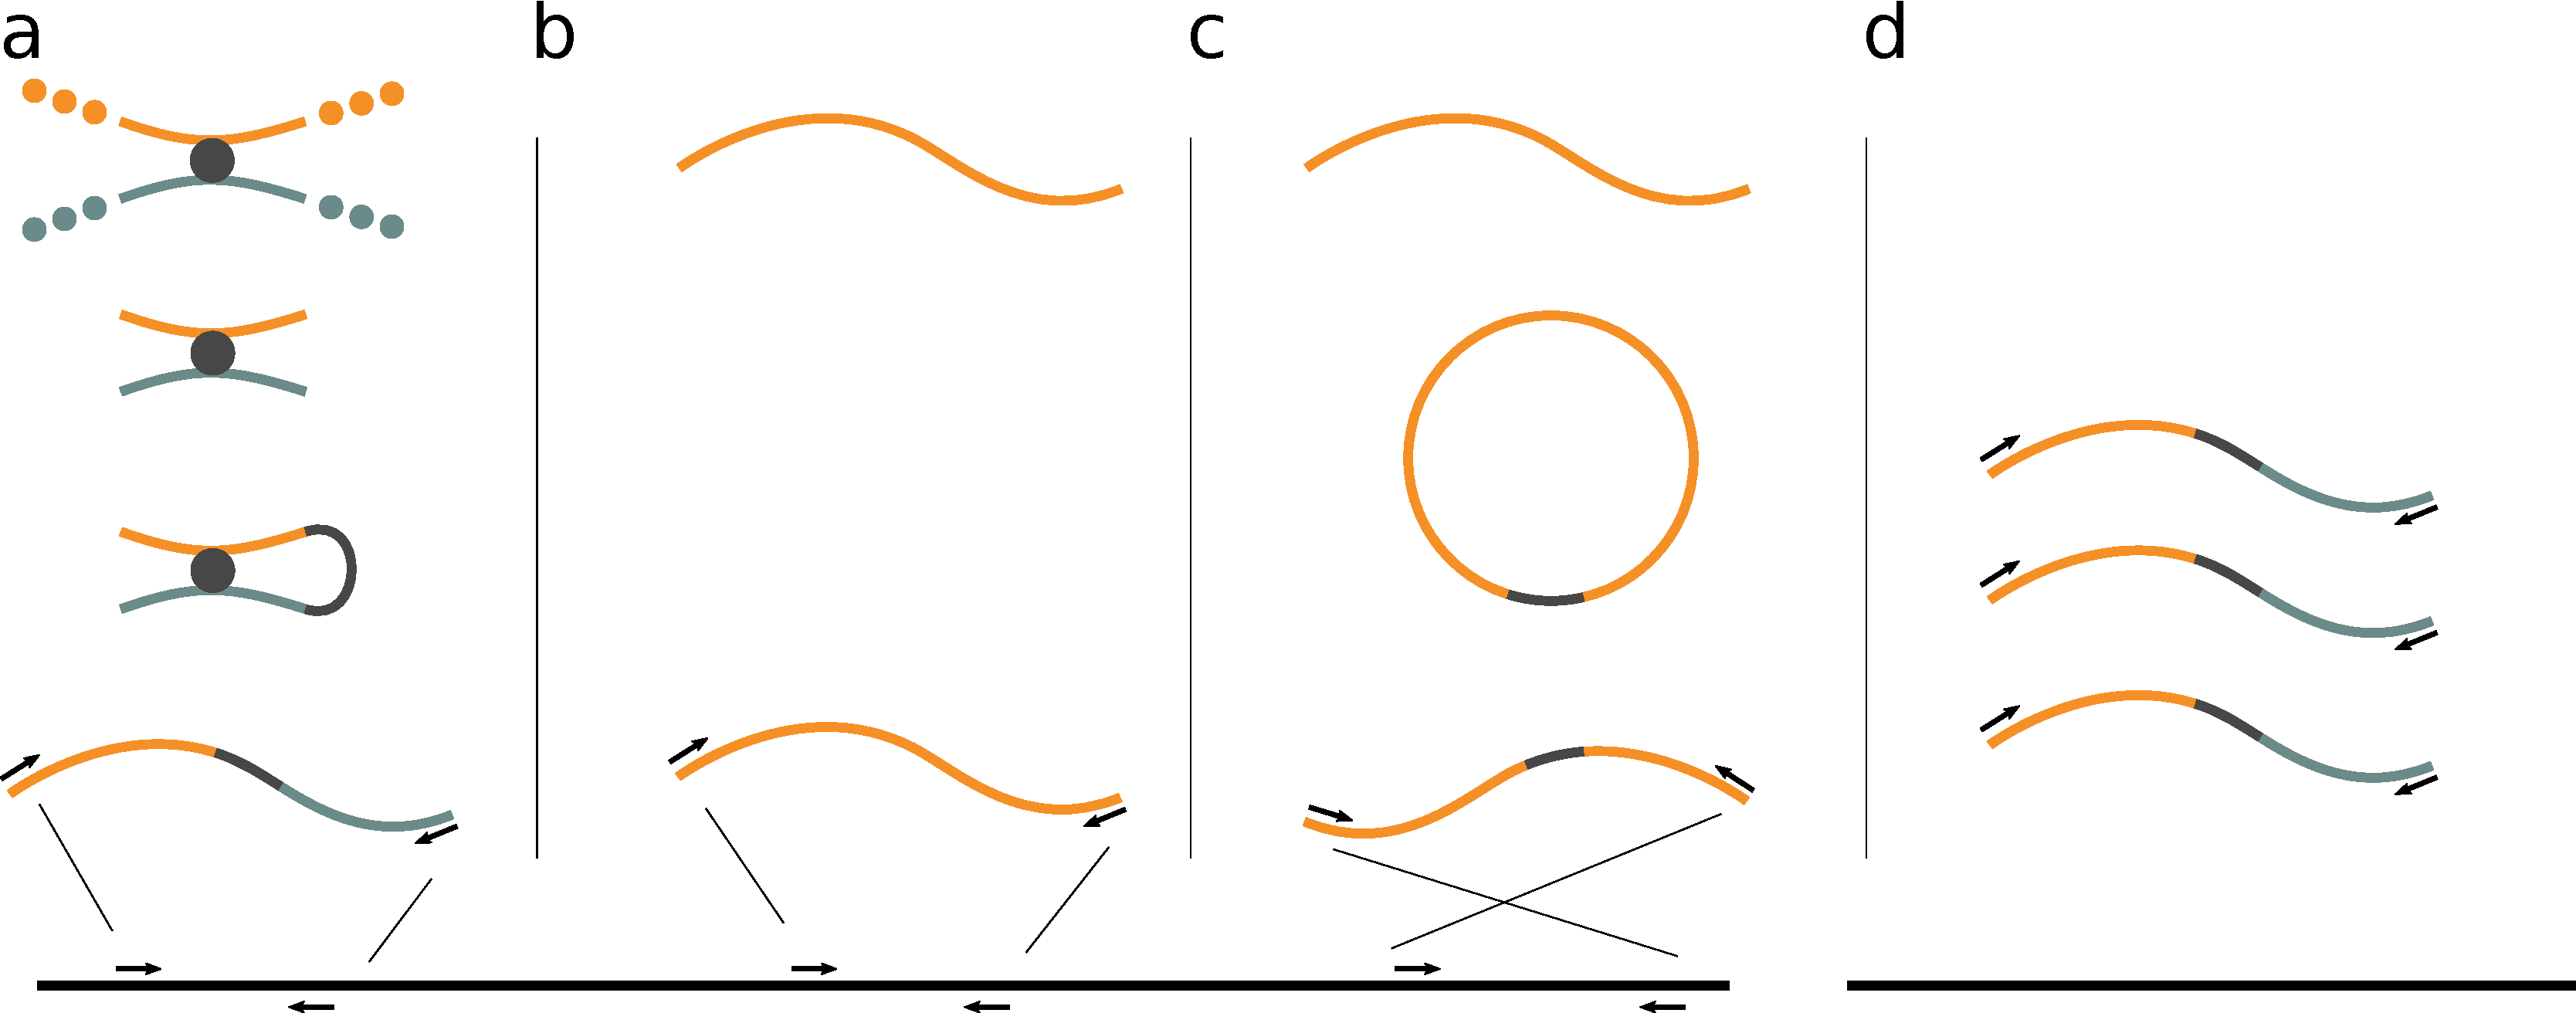
\includegraphics[width=\textwidth]{Parts/Part02/gfx/hicstuff/filters.pdf}
    \caption[Types of interactions generated from Hi-C experiments.]{Types of interactions generated from Hi-C experiments: \textbf{a:} Valid interaction resulting from the religation of two distant loci in physical contact. \textbf{b:} Spurious event caused by the sequencing of a single restriction fragment, or undigested sequence. \textbf{c:} Spurious event resulting from the self-religation and breakage of a fragment. \textbf{d:} Interactions caused by PCR duplicates. Both reads have the exact same coordinates for all PCR duplicate pairs.}
    \label{fig:02-01:filters}
\end{figure}

These biases must be accounted for when processing Hi-C data. This can be achieved by identifying and filtering out faulty interactions based on their strands.

This preprocessing is often performed using custom scripts and prone to errors, bugs and lack of informations about parameters. In an effort to improve reproducibility and accessibility of Hi-C analysis, we developed hicstuff, an open source Hi-C pipeline that incorporate all the aforementioned steps, along with several downstream processing utilities (Fig. \ref{fig:02-01:pipeline}).

\begin{figure}[htb]
    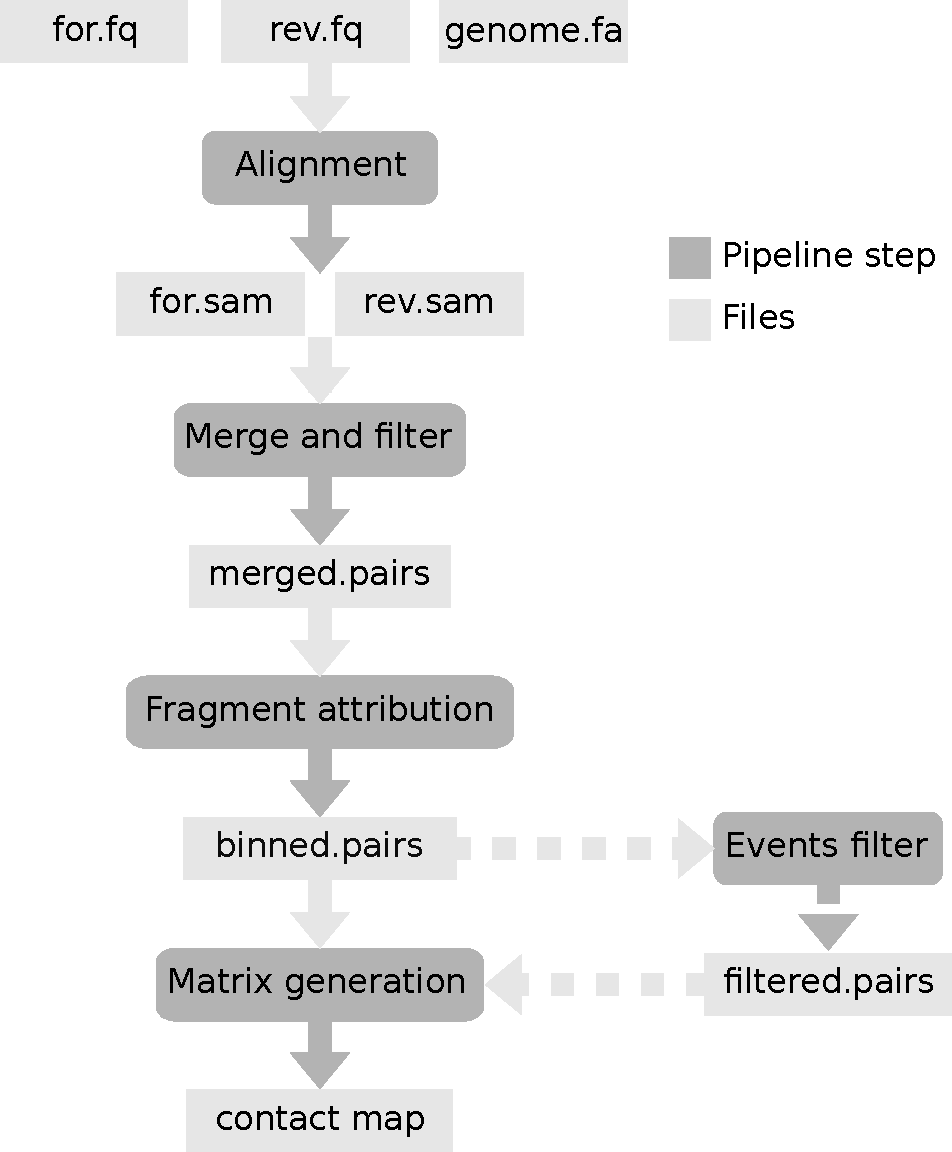
\includegraphics[width=0.7\textwidth]{Parts/Part02/gfx/hicstuff/pipeline.pdf}
    \caption[Overview of the hicstuff pipeline.]{Overview of the hicstuff pipeline: Consecutive steps towards the generation of a contact map from sequencing reads, along with the intermediate files are shown as a directed acyclic graph.}
    \label{fig:02-01:pipeline}
\end{figure}

Hicstuff can properly align chimeric reads, by digesting them \textit{in-silico} at religation sites, or using iterative mapping (Fig. \ref{fig:02-01:iteralign}) where reads are truncated and iteratively extended until they align unambiguously. The Hi-C pairs are then assigned a numerical index according to the restriction fragment they originate from (Fig. \ref{fig:02-01:attribution}) and artifactual contacts are filtered out using the strand information. Contacts in each bin combination are then summed into a "contact matrix", which is stored in sparse format to spare memory (Fig. \ref{fig:02-01:sparse}). To allow compatibility with various programs, it can generate sparse matrices in 3 possible formats: COO, bedgraph2d and cool. COO (COOrdinate format) and bedgraph2D are text-based sparse matrix representations, while cool \cite{abdennurCoolerScalableStorage2020} is a specification based on the binary HDF5 (hierarchical data format) to represent Hi-C data. The cool format is seeing widespread adoption in the research community and offers several advantages, including low storage space, ease of use and fast random access compared to text formats.

\begin{figure}[htb]
    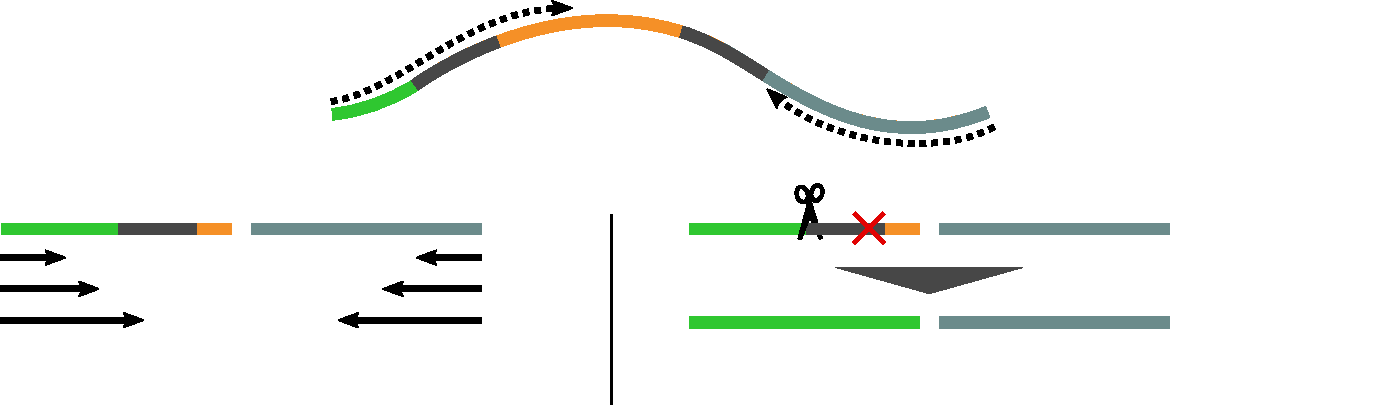
\includegraphics[width=1\textwidth]{Parts/Part02/gfx/hicstuff/iteralign.pdf}
    \caption[Iterative alignment of a Hi-C pair.]{Iterative alignment of a Hi-C pair: The Hi-C fragment consists of 3 regions religated together (top). One sequencing read spans two regions (orange and green). Iterative alignment is used to uniquely align the resulting chimeric read (left). The read is truncated to a short length (e.g. 20bp) and iteratively extended until it aligns to a unique position in the genome. Alternatively, reads which do not map uniquely can be digested \textit{in-silico} at known religation sites (right) to remove the chimeric part. The digested reads are then realigned.}
    \label{fig:02-01:iteralign}
\end{figure}

\begin{figure}[htb]
    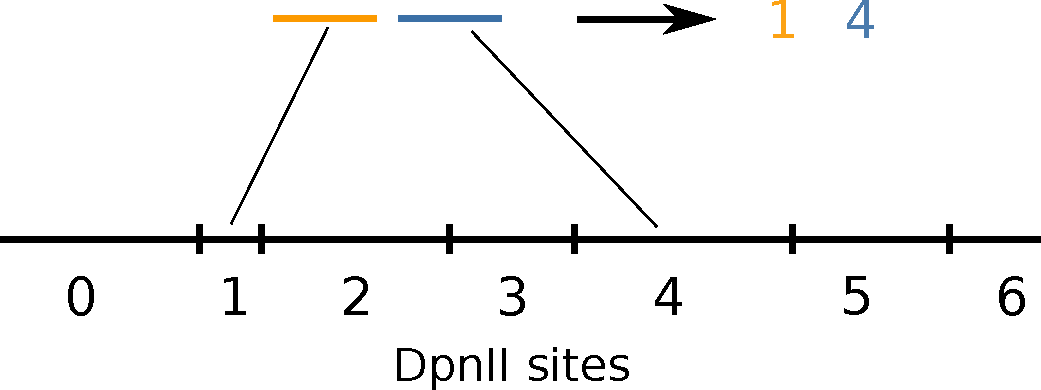
\includegraphics[width=0.8\textwidth]{Parts/Part02/gfx/hicstuff/hic_pipeline_attribution.pdf}
    \caption[Fragment attribution of Hi-C contacts.]{Fragment attribution of Hi-C contacts: The genome is segmented into discrete bins according to the positions of restriction sites. Hi-C reads are assigned an index according to the restriction fragment to which they aligned.}
    \label{fig:02-01:attribution}
\end{figure}

\begin{figure}[htb]
    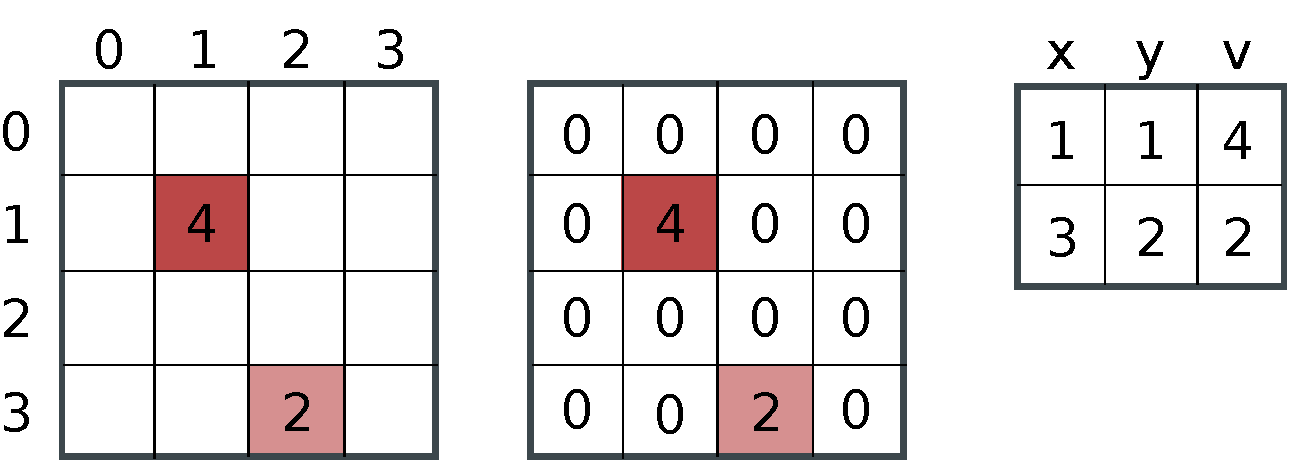
\includegraphics[width=\textwidth]{Parts/Part02/gfx/hicstuff/dense_sparse.pdf}
    \caption[Dense and sparse matrix representations.]{Dense and sparse matrix representations: . In Hi-C, matrices are very sparse (i.e. mostly contain 0s), (left). In dense matrix representation, we store all values explicitely. The information stored is highly redundant (middle). Such matrices can be stored efficiently using a sparse representation where only non-zero values are stored explicitely along with their coordinates (right).}
    \label{fig:02-01:sparse}
\end{figure}

Hicstuff is meant to be easily accessible \cite{matthey-doretSimpleLibraryPipeline2021}, even to non-expert users. It has a comprehensive online documentation and tutorials, and the program and its dependencies are installed with a single command. The program is written in python and is accessible both via a \acrfull{CLI} to use it as an executable, and an \acrfull{API} to import it as a python library. It is covered by unit tests which are automatically executed on each new release, on the cloud through a continuous integration service to reduce the likelihood of bugs. Hicstuff runs well with default parameters, but has many options to fit most common use cases. It works regardless of genome size or organism.

The pipeline also provides reproducibility through an automatic logging of every intermediate result in the pipeline as well as the input parameters used.

The project has already fostered a modest community of users which are offering their contributions, suggest features or report issues they encounter. The Hicstuff pipeline is distributed through the python package index (PyPI) and its source code is available on github: \url{https://github.com/koszullab/hicstuff}.

\FloatBarrier
\section{Feature detection with Chromosight}

The downstream analysis of chromosome contact maps often involves looking for signals reflecting biologically relevant spatial interactions. Several specialized approaches for pattern detection have been proposed in the past \cite{sergeyvenevOpen2cCooltoolsV02021,wolffLoopDetectionUsing2020,rao3DMapHuman2014}. Each of these methods use a set of specific rules to detect one particular type of pattern. For example, HICCUPS \cite{rao3DMapHuman2014} detects chromatin loops by scanning each pixel of the contact map for contact enrichment compared to surrounding pixels.

These specialized methods present several drawbacks, including strong reliance on parameter values, poor generalization to non-model species and poor detection rates. These shortcomings motivated us to work on a more generalized pattern detection method to identify arbitrary patterns in chromosome contact maps. We developed a python package  named \textit{Chromosight}, which performs pattern detection on Hi-C matrices in cool format.

Chromosight uses template matching to identify features on a chromosome contact map. This technique consists in scanning the input Hi-C matrix with a smaller "kernel" image corresponding to the pattern of interest (e.g. a loop) to identify input regions bearing similarity to the kernel. This has the added benefit of allowing to swap the kernel to detect a different feature.

One of the main algorithmic challenges of applying a convolution-based method to Hi-C data is the size of matrices. Hi-C matrices are notoriously large, but they are also extremely sparse (most loci do not interact with each other). As a consequence, sparse matrix representation is generally used to handle Hi-C data (Fig. \ref{fig:02-01:sparse}). In the case of large genomes, such as that of \textit{Homo sapiens}, an entire chromosome's contact can consist of to 30,000 x 30,000 bins of 10 kbp. One of the main drawbacks of sparse representation is that most algorithms are slower and harder to implement on such structures. No implementation of convolution for sparse matrices was openly available, which prompted us to write an efficient method to scan the billion of pixels from Hi-C maps in reasonable time. Fortunately, the convolution problem can be reformulated as a matrix multiplication by transforming the input matrices (see \ref{sec:04-A-01:convolution}), and matrix multiplication is a standardized operation that has been highly optimized in low level libraries, including for sparse matrices.

During the development of Chromosight, we put special attention on good software practices mentioned in section \ref{sec:02-01:streamlined-processing} to make it easy to use and accessible. This was done by spending time documenting the python \acrshort{API} and the \acrshort{CLI} as well as publishing publicly accessible tutorials and examples on a dedicated readthedocs website (\url{https://www.chromosight.readthedocs.io/}). Furthermore, the program is covered by a suite of unit tests set up with continuous integration. On every new release, Chromosight is automatically distributed on PyPI, bioconda and dockerhub to accomodate the different use cases and pipelines.

Chromosight's algorithm, results and benchmark against state of the art loop detection methods are presented in details in the following pages. The algorithmic details used to tackle the sparse convolution problem are presented in Appendix \ref{sec:04-A-01:convolution}. Additionally, a case study demonstrating Chromosight capabilities is shown in appendix \ref{ch:04-B:demo}.

\includepdf[pages=-,addtotoc={
     2,subsection,2,Introduction,sec:02-01:chromo-int,   
     3,subsection,2,Results,sec:02-01:chromo-res,
     8,subsection,2,Discussion,sec:02-01:chromo-dis,
     8,subsection,2,Methods,sec:02-01:chromo-met,
     12,subsection,2,Supplementary information,sec:02-01:chromo-sup}]
     {Publications/chromosight_publication_supp.pdf}    

\section{Change detection across biological conditions}

Change detection is a classic problem in the field of signal processing and remote sensing. Given two or more input signals such as images, one wants to identify the portions that differ between them. This problem also applies to Hi-C contact maps, where it natural to want to detect regions of contact maps that differ between biological conditions, indicating changes in the organization of chromosomes. Importantly, the significance of these differences have to be assessed, given the sparsity of many areas of the contact maps (especially between DNA segments separated by long distances in \textit{cis}).

Several computational solutions have been developed to tackle this challenge. Some of them, such as diffhic \cite{lunDiffHicBioconductorPackage2015}, formulate the problem similarly to a differential expression RNAseq analysis using contact counts instead of read counts. This approach has the benefit of being straightforward, however it only finds non-specific variations in the amount of contacts. These variations can reflect specific spatial interactions, but also differential compartment switches or insulation changes, which could be caused by a number of different phenomena.

When I started working on Hi-C data, there was therefore a need for a program that would detect significant changes in contact maps with a focus on specific chromatin features. We developed pareidolia\footnote{Pareidolia: From Ancient Greek {\textgreekfont παρα} (para, "alongside, concurrent") + {\textgreekfont εἴδωλον} (eídōlon, "image"): the tendency to interpret a vague stimulus as something known to the observer, such as interpreting marks on Mars as canals, seeing shapes in clouds, or hearing hidden messages in music.}, a software package for change detection with an a priori on the type of signal to detect. The method is "supervised" in the sense that it requires a kernel representing the feature of interest. Pareidolia relies on Chromosight's convolution engine to convert the contact map of each condition into a map of correlation coefficients representing similarity with the feature of interest. Change detection is then performed on these coefficients. As a consequence, rather than looking for contacts increase, pareidolia looks for changes in feature similarity, such as border sharpness or looping intensity.

\subsection{Pareidolia algorithm}

Pareidolia works by comparing one or several samples issued from two conditions such as treatments or timepoints.

% Could add preprocessing of missing bins and uniformization of sparsity structure

Assuming two conditions $t=\{t_0, t_1\}$, each with multiple biological samples (replicates) $r=\{r_1, r_2, ..., r_R\}$. The whole genome contact matrix from each sample $H_{r, t}^{n \times n}$ is first processed using Chromosight's convolution algorithm as described in \ref{sec:02-01:chromo-met} to generate a matrix of similarity $M_{r, t}^{n \times n}$ with kernel $K$ representing the pattern of interest. In the resulting matrix, the value at position (i, j), thereafter denoted $M_{r, t}[i, j]$, is a Pearson correlation coefficient with $K$, therefore $M_{r,t}[i, j] \in [-1, 1]$.

Change detection is applied using an algorithm inspired by median filtering-based background formation \cite{ilseverTwoDimensionalChangeDetection2012} (Fig. \ref{fig:02-01:pareidolia}). First, we generate a background matrix $B_t$ for each condition (timepoint), whose values are defined as the median of all replicates' Chromosight correlation maps from that condition (Eq. \ref{eqn:02-01:pareidolia-bg}). The change matrix $D$ is then obtained by taking the difference between condition backgrounds (Eq. \ref{eqn:02-01:pareidolia-diff}). Note that, although values in $B_t$ and $D$ are computed independently at each position [i, j], the spatial dependency between values is taken into account through the convolution operation used to produce $M_{r, t}$.

\begin{align}
    \label{eqn:02-01:pareidolia-bg}
    B_t[i, j] &= median(M_{1, t}[i, j], M_{2, t}[i, j], ..., M_{R, t}[i, j]) \\
    \label{eqn:02-01:pareidolia-diff}
    D[i, j] &= B_{t_1}[i, j] - B_{t_0}[i, j]
\end{align}

We then compute the matrix of standard errors $S$ between each replicate and their condition's median background (Eq. \ref{eqn:02-01:pareidolia-se}). This technical variability (among replicates) is then used to filter out noisy regions. This is done by generating a \acrfull{CNR} map $C$ (Eq. \ref{eqn:02-01:pareidolia-cnr}) and applying a threshold to it. This matrix represents the ratio of contrast (inter-condition difference) over noise (intra condition variability).

\begin{align}
    \label{eqn:02-01:pareidolia-se}
    S &= \frac{1}{T}\sum_{t=0}^T{\sqrt{\frac{1}{R}\sum_{r=1}^R{(M_{r, t} - B_t)^2}}} \\
    \label{eqn:02-01:pareidolia-cnr}
    C   &= \frac{\left|B_{t_1} - B_{t_0}\right|}{S}
\end{align}

Three coordinates sets are then defined to select regions of interest for change detection:
\begin{itemize}
    \item Positions with a local contact density above $T_d$. If a kernel $K$ of size $m_K \times n_K$ is used to compute $M$, the local contact density $L$ is defined as the proportion of nonzero contact values within a window of $m_K \times n_k$ centered on $H[i, j]$ (Eq. \ref{eqn:02-01:local-density}). Each position must be above a threshold in all biological samples to be considered (Eq. \ref{eqn:02-01:filter-d}). This set is used to select for sufficient coverage.
    \item Positions for which at least one biological sample from either condition has a Chromosight score above threshold $T_p$ (Eq. \ref{eqn:02-01:filter-p}). This set is used to select for clear patterns.
    \item Pixels in regions with a \acrshort{CNR} above threshold $T_c$ (Eq. \ref{eqn:02-01:filter-c}). This set is used to select for high contrast between conditions.
\end{itemize}

The required thresholds $T_c$, $T_p$ and $T_d$ are provided with default values but can also be set by the user. The intersection $F$ of the 3 resulting coordinate sets is then computed (Eq. \ref{eqn:02-01:filters}) and the change matrix $D$ is filtered to retain only coordinates present in $F$ (Eq. \ref{eqn:02-01:filter-diff}), effectively retaining change values passing all conditions and setting others to 0.

\begin{align}
    \label{eqn:02-01:local-density}
    L_{r,t}[i, j] &= \sum_{x=1}^{m_K} {\sum_{y=1}^{n_K}{(1 - \delta(0, H_{r, t}[i+x - \frac{m_K+1}{2}, j+y-\frac{n_K+1}{2}]))}} \\
    \intertext{where $\delta(a, b)$ is the Kronecker delta:}
    \delta(a, b) &= \begin{cases} \nonumber
        0, & a \neq b \\
        1,  & a = b \\
    \end{cases}
\end{align}

\begin{align}
    \label{eqn:02-01:filter-d}
    F_d &= \{ (i, j) \mid \min_{r \in R}{L_{r, .}[i, j]} \geq T_d \} \\
    \label{eqn:02-01:filter-p}
    F_p &= \{ (i, j) \mid \max_{r \in R}{M_{r, .}[i, j]} \geq T_p \} \\
    \label{eqn:02-01:filter-c}
    F_c &= \{ (i,j) \mid C[i,j] > T_c \} \\
    \label{eqn:02-01:filters}
    F   &= F_c \land F_p \land F_d \\
    \label{eqn:02-01:filter-diff}
    D_f[i, j] &= 
    \begin{cases}
        D[i, j], & (i, j) \in F \\
        0, & otherwise \\
    \end{cases}
\end{align}

\begin{figure}[htb]
    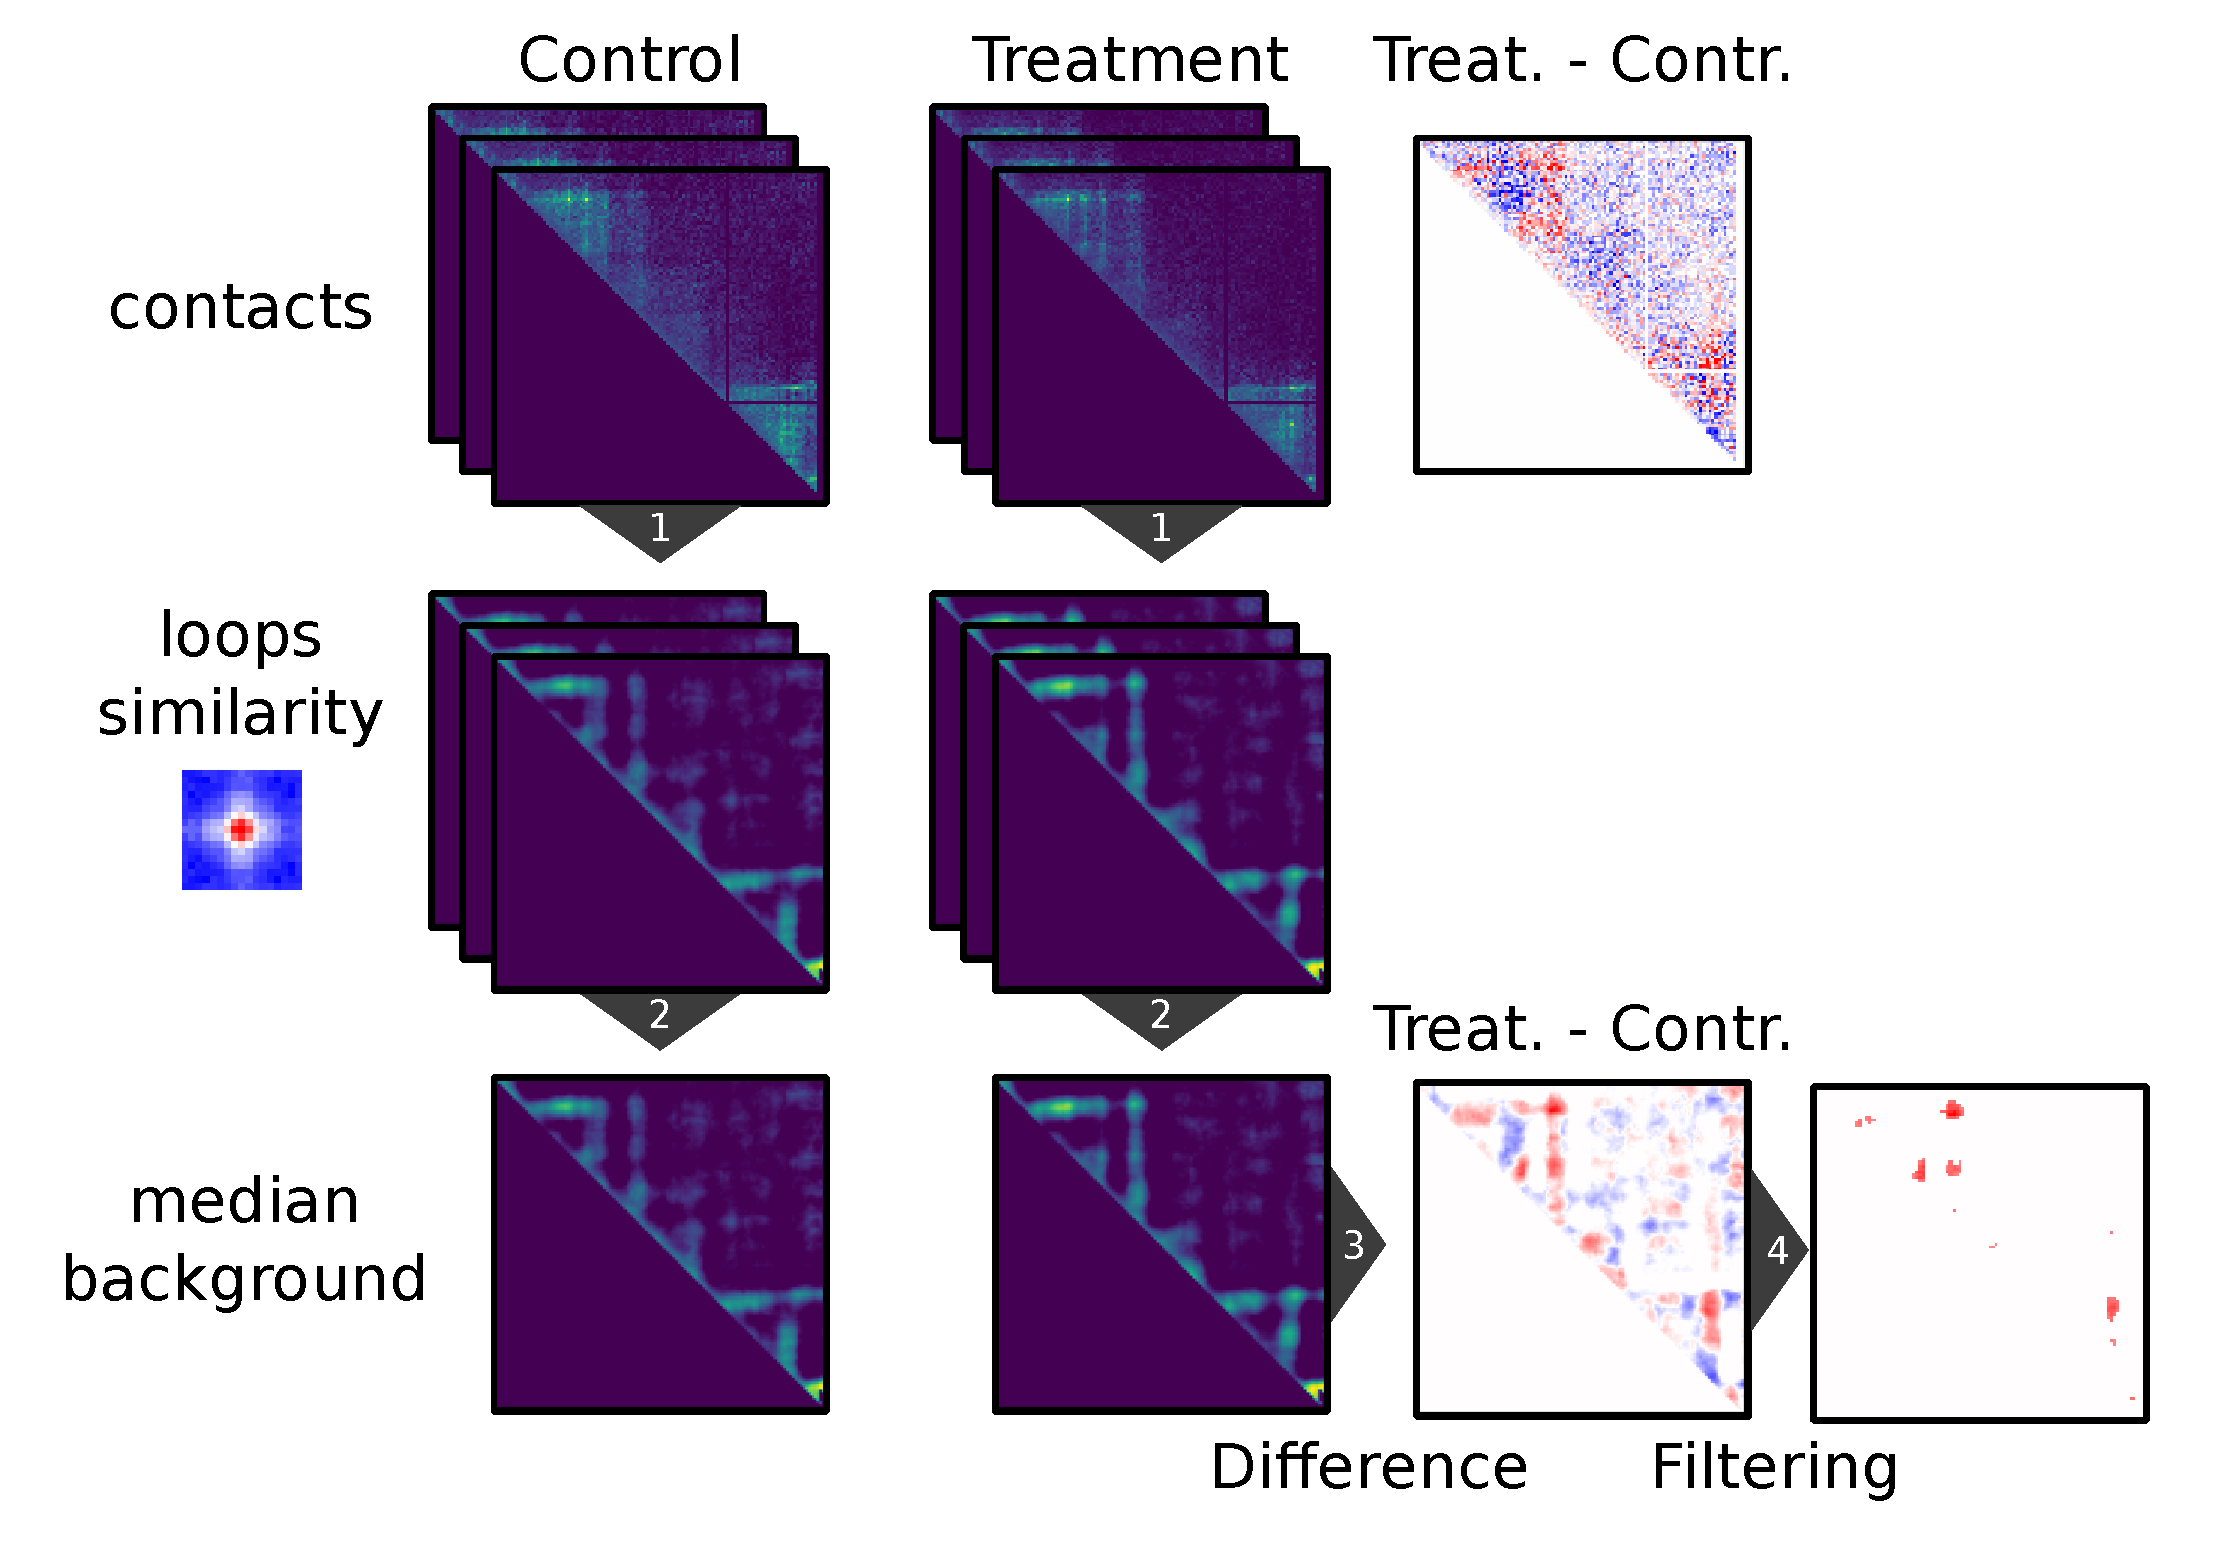
\includegraphics[width=\textwidth]{Parts/Part02/gfx/pareidolia_process.pdf}
    \caption[Pareidolia algorithm.]{Pareidolia algorithm. From top to bottom: The Hi-C contact maps of several replicates ($r$) in two conditions ($t_0, t_1$) are shown, as well as the difference between conditions. Chromosight's convolution algorithm is used on each sample \textbf{1} to generate a map of correlation coefficients ($M$) with the kernel of interest (loops in this case). For each condition, a median background ($B$) is computed among replicates \textbf{2}. The difference between these two backgrounds ($D$) is then extracted \textbf{3} and filtered \textbf{4} using a combination of \acrshort{CNR}, contact density and pattern intensity thresholds to obtain the final change matrix ($D_f$).}
    \label{fig:02-01:pareidolia}
\end{figure}

Pareidolia can either return the pattern intensity changes $D_f$ at a set of predetermined $(i, j)$ positions provided as input, or perform a \textit{de-novo} detection of differential loops on the Hi-C map. For \textit{de-novo} detection, pareidolia applies Chromosight's implementation of the connected component labelling algorithm for sparse matrices, described in \ref{sec:02-01:chromo-met}. This operation isolates contiguous foci of non-zero differential changes in $D_f$ and retrieve the local absolute maximum in each focus. The list of coordinates along with their respective differential intensity score is returned.

The inner steps of Pareidolia are further detailed with visual representations of the intermediate matrices and filters on experimental data in Appendix \ref{ch:04-C:pareidolia}.

\subsection{Results on experimental data}

To showcase the use of Pareidolia, we used it to measure loop changes upon depletion of CTCF in murine cells using published data \cite{noraTargetedDegradationCTCF2017}. CTCF acts as a roadblock for the motor protein cohesin which travels along the chromatin fiber. Cohesin accumulates at CTCF binding sites, forming stable chromatin loops between pairs of CTCF binding sites.

These looping interactions have been shown to be weakened or disappear in the absence of cohesin \cite{raoCohesinLossEliminates2017} or CTCF \cite{noraTargetedDegradationCTCF2017}. Here we show an example use of Pareidolia to quantify these 3D changes.

The dataset consists of CTCF-AID mutant mouse embryonic stem cells (ES-E14TG2a). When auxin treatment is applied, the CTCF-AID recombinant protein is degraded. We use pareidolia to compare chromatin loops before and after auxin treatments, using 2 replicates per condition.

With default parameters, pareidolia identifies a total of 2,997 disappearing differential loops and 845 appearing loops (Fig. \ref{fig:02-01:pareidolia-experimental}).

\begin{figure}[htb]
    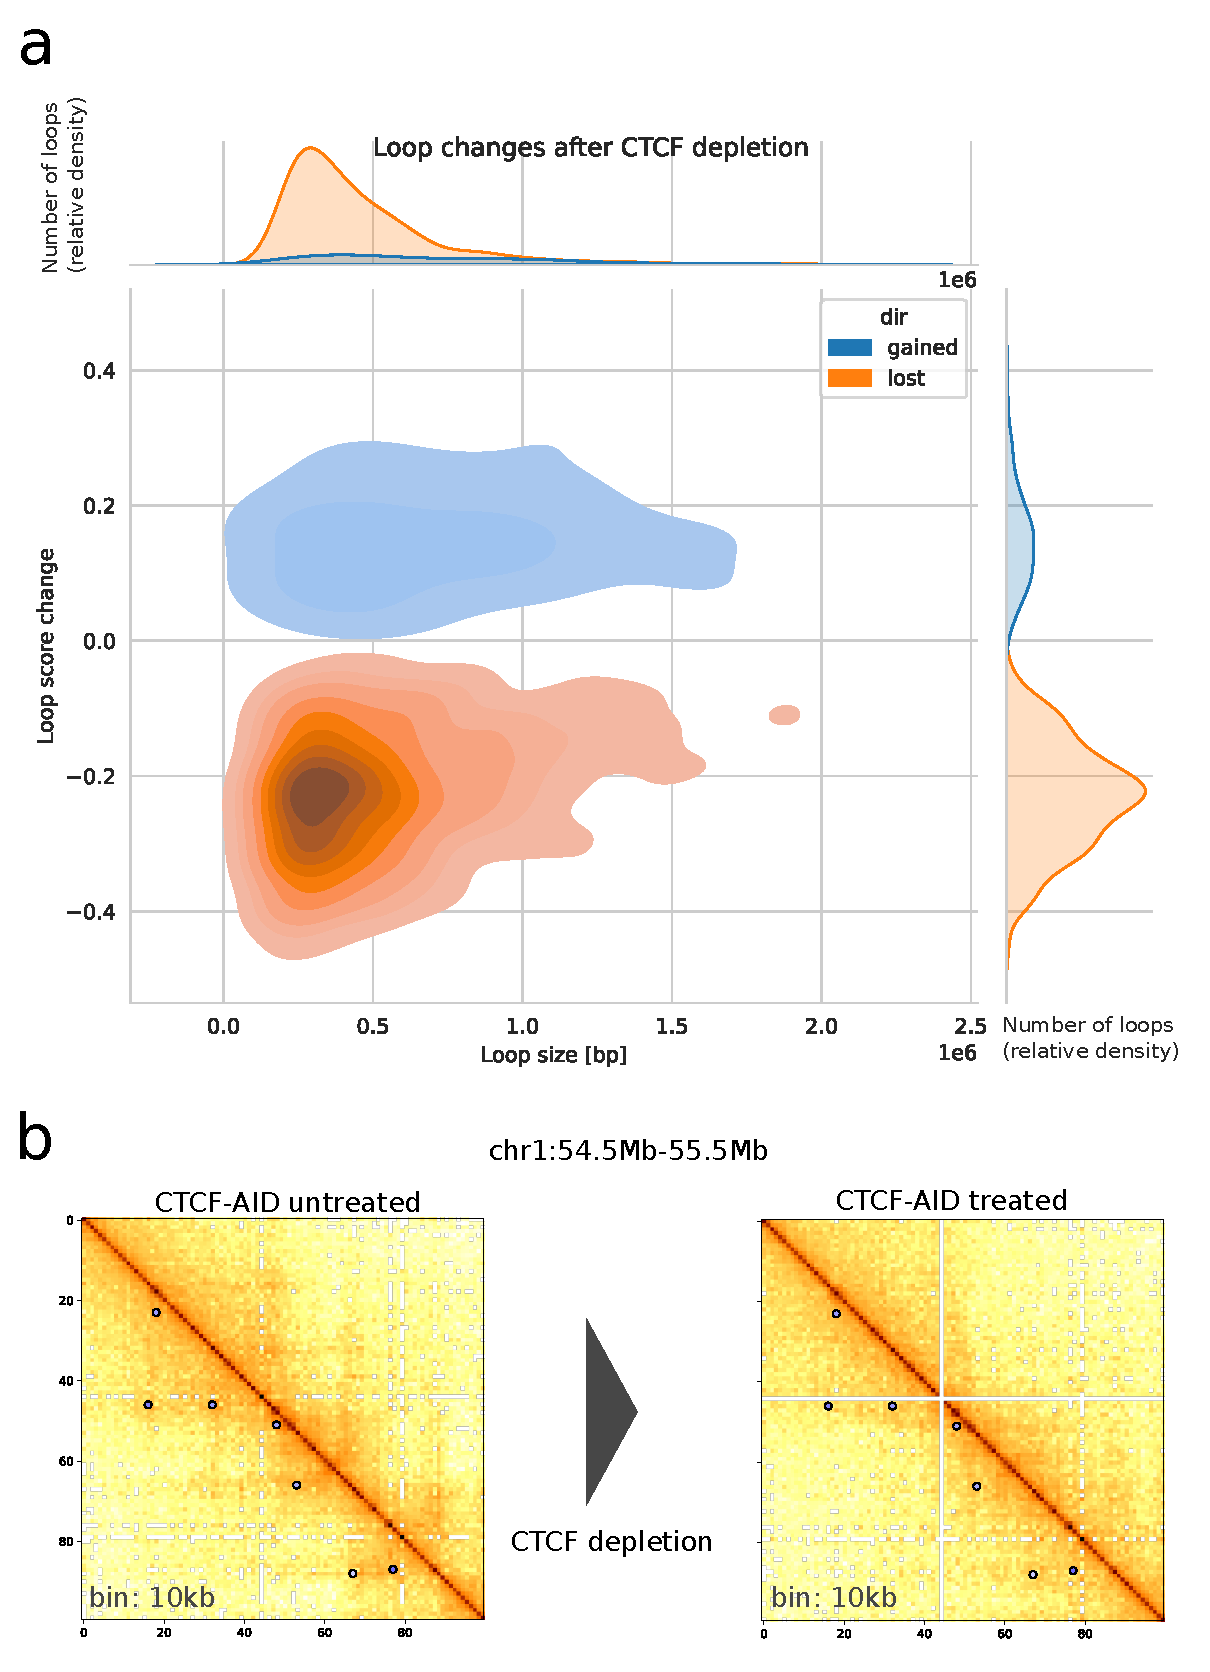
\includegraphics[width=\textwidth]{Parts/Part02/gfx/pareidolia/ctcf_depletion_scores_genome.pdf}
    \caption[Pareidolia results on CTCF degradation experiments.]{Pareidolia results on CTCF degradation experiments from \cite{noraTargetedDegradationCTCF2017}: \textbf{a:} Distribution of chromatin loop change and size upon CTCF depletion as detected by pareidolia. \textbf{b:} Zoom on a region of the Hi-C map from mouse chromosome 1. Disappearing loops detected by pareidolia are highlighted in blue. For visualization purpose, replicates were merged in Hi-C matrices shown. Processed data retrieved from \url{https://data.4dnucleome.org}, accessions 4DNES87HWQAX and 4DNES7UKQHOX.}
    \label{fig:02-01:pareidolia-experimental}
\end{figure}

\subsection{Perspectives and potential improvements}

Pareidolia is one of the few available computational methods for differential Hi-C analysis which leverages replicates \cite{lunDiffHicBioconductorPackage2015,stansfieldMultiHiCcompareJointNormalization2019,sahinHiCDCEnablesSystematic2021,djekidelFINDDifFerentialChromatin2018,cookMeasuringSignificantChanges2020}. While these methods focus on differential contact enrichment, often through fitting a Poisson or negative binomial model, Pareidolia detects change relative to a predefined pattern. In the case of Hi-C data, we estimated that this was a proper solution, given the emphasis of most if not all investigations on limited number of specific chromatin features such as loops, stripes, etc. On the other hand, one may miss some unexpected changes in some conditions, but these cases remain rare. Pareidolia is computationally efficient due to the use of sparse matrices throughout the program and maximal use of vectorized operations. Although a formal benchmark has yet to be performed, its core functionality relies on Chromosight which has been thoroughly evaluated, and gives promising results on empirical tests.

Although Pareidolia currently supports only two condition, the code was written with the intent of being extended to multiple conditions or timepoints. This would most likely involve a different change metric than background accumulation, such as a regression, but could be implemented with relatively few modifications to the code. A limitation of Pareidolia is the reliance on threshold values to filter noise and filter differences. It could be possible to solve this issue by automatically selecting thresholds based on the distribution of contacts and similarity scores in the input samples.